\documentclass[12pt]{scrartcl}

\usepackage{amsmath,amssymb}
\usepackage{fullpage}
\usepackage{enumitem}
\usepackage{hyperref}
\usepackage{graphicx}
\usepackage{tikz}
\usepackage{pgfplots}
\usepackage{float}
\usepackage{tabularx}
\usepackage{titlesec}

\pgfplotsset{compat=1.18}
\usetikzlibrary{trees,positioning,shapes,arrows}
\usepgfplotslibrary{statistics} 
\setlength{\parindent}{0pt}

\tikzset{
  basic/.style  = {draw, text width=2cm, drop shadow, font=\sffamily, rectangle},
  root/.style   = {basic, rounded corners=2pt, thin, align=center, fill=white},
  level-2/.style = {basic, rounded corners=6pt, thin,align=center, fill=white, text width=3cm},
  level-3/.style = {basic, thin, align=center, fill=white, text width=1.8cm}
}

\titleformat{\section}  % which section command to format
{\fontsize{12}{14}\bfseries} % format for whole line
{\thesection} % how to show number
{1em} % space between number and text
{} % formatting for just the text
[] % formatting for after the text

\titleformat{\subsection}  % which section command to format
{\fontsize{12}{14}\bfseries} % format for whole line
{\thesubsection} % how to show number
{1em} % space between number and text
{} % formatting for just the text
[] % formatting for after the text

\begin{document}

\begin{center}
	\hrule
	\vspace{0.4cm}
	{\textbf{\large Lecture 02: Probability Theory}}\\ [0.2cm]
	INF1004 Mathematics II

\end{center}

\textbf{Name:} Timothy Chia \hspace{\fill} \textbf{Date:} 12/01/2025 \\

\hrule

\section{Types of Probability}
Probability is defined as a number in the range $[0,1]$ that is assigned to an event associated with a random experiment. There are two interpretations of probability theory that guide how such values are assigned:

\subsection{Classical Probability}
In classical probability, all outcomes in the sample space are assumed to be equally likely.\\
The probability of a random event $A$ occuring is given as $$P(A)=\frac{\text{Number of different outcomes in A}}{\text{Total number of possible outcomes}}$$
\textbf{\textit{Note:}} This definition is not very practical for everyday life because it assumes the outcomes are equally likely.

\subsection{Empirical Probability}
In empirical probability theory, the probability of an event $A$ occurring  approximated by the relative frequency of its occurrence over a large number of trials such that $$P(A)=\frac{\text{Number of times an outcome occurs}}{\text{Total number of observations}}$$
This interpretation relies on collecting data over the years or existing historical data to propose such relative frequencies.

\subsection{Definitions}
\begin{itemize}
	\item We define a sample space $S$ as the set of all possible outcomes of a random phenomenon.
	\item An event $A$ is defined as the set of outcomes under investigation.
	\item By definition of probability, the following statements must hold to be valid: $$0 \leq P(A) \leq 1,\ P(S)=1$$
	\item If $A_1, A_2, \ldots$ are mutually exclusive events, then $$P\!\left(\bigcup_{i} A_i\right) = \sum_{i} P(A_i)$$.
\end{itemize}

%------------------------------------------------------------
\newpage
\section{Complementary Events}
The complement of an event $A$ denoted $P(A^c)$ and is given by $$P(A^c) = P(S) - P(A)$$

Conceptually, the complement of an event can be thought of as the probability that it does not occur. Visually, this can be represented as the area in a venn diagram that is not in $A$.

\begin{center}
	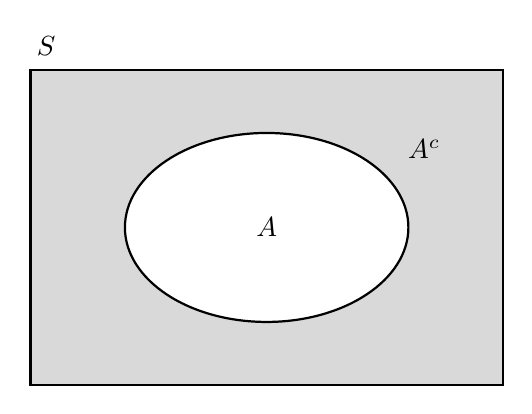
\begin{tikzpicture}
		% Sample space S
		\draw[thick, fill=gray!30] (0,0) rectangle (6,4);
		\node at (0.2,4.3) {$S$};

		% Event A
		\draw[thick, fill=white!30] (3,2) ellipse (1.8cm and 1.2cm);
		\node at (3,2) {$A$};

		% Complement label
		\node at (5,3) {$A^{c}$};
	\end{tikzpicture}
\end{center}

\section{Intersection of Events}
Given two events $A$ and $B$, the probability of their intersection denoted $$P(A \cap B)$$ is the probability that both events occur. In a venn diagram, it is the area where both events overlap.

\begin{center}
	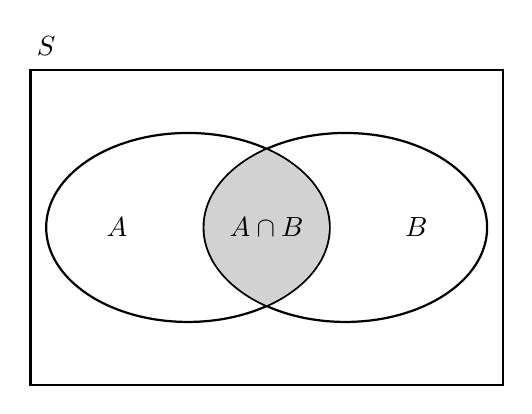
\begin{tikzpicture}
		% Sample space
		\draw[thick] (0,0) rectangle (6,4);
		\node at (0.2,4.3) {$S$};

		% Circles/ellipses outlines (unfilled)
		\draw[thick] (2,2) ellipse (1.8cm and 1.2cm);
		\draw[thick] (4,2) ellipse (1.8cm and 1.2cm);


		% Shade intersection only (clip trick)
		\begin{scope}
			\clip (2,2) ellipse (1.79cm and 1.19cm);
			\fill[gray!35] (4,2) ellipse (1.79cm and 1.19cm);
		\end{scope}

		% Labels
    \node at (1.1,2) {$A$};
    \node at (4.9,2) {$B$};
		\node at (3,2) {$A \cap B$};
	\end{tikzpicture}
\end{center}

If two events $A$ and $B$ are mutually exclusive, then $P(A \cap B) = 0$ because both events never overlap.

\section{Union of Events}

%------------------------------------------------------------
\newpage
\section{Inclusion-Exclusion Principle}

%------------------------------------------------------------
\newpage
\section{Multiplicative Rule of Probability}

%------------------------------------------------------------
\newpage
\section{Independent and Mutually Exclusive Events}

%------------------------------------------------------------
\newpage
\section{Law of Total Probability}

%------------------------------------------------------------
\newpage
\section{Bayes' Theorem}

\end{document}
